\chapter[Introduction]{Introduction}

In the coming century we face a loss of biodiversity on the order of 100--10,000 times greater than average rates in the fossil record \citep{mea2005} --- a rate as fast if not faster than any of the five past mass extinctions \citep{barnosky2011, harnik2012}. Compounding this problem for conservation managers is uncertainty in future climate conditions \citep{heller2009} and the unknown responses of species and communities to those conditions \citep{lavergne2010}. Therefore, urgent questions are: Exactly how big a problem is the loss of biodiversity for the stability of ecological systems? How can conservation biologists communicate the insurance benefit of biodiversity to the public and policy makers? And, how can we apply limited conservation funds to manage biodiversity and limit risk in the face of increasing environmental uncertainty?

Nearly a decade ago, \citet{figge2004} and \citet{koellner2006} laid the foundation for why financial portfolio theory is ideally suited for answering these questions. Financial portfolio theory seems applicable to ecological systems for at least four reasons. First, ecological and financial systems are both structured hierarchically. Groups of populations form metapopulations and groups of species form communities; groups of financial assets form investment funds, which in turn form portfolios. Additionally, ecological and financial managers have similar goals. Ecological resource managers might wish to minimize the probability of population decline while maintaining an acceptable level of hunting of fishing; financial portfolio managers minimize the probability of large economic losses for an acceptable level of expected financial returns \citep{may2008}. Another reason why portfolio theory is ideally suited for ecology is that substantial resources have gone into developing mathematical theory for optimizing financial investments. There is therefore a rich body of theory and experience to draw from. Finally, the portfolio metaphor is an engaging and accessible way for ecologists and conservationists to think about ecological variance and biological diversity and convey the importance of this (often abstract) literature.

A number of recent studies have used financial portfolios as a metaphor, metric, or management approach (Fig.~\ref{fig:traits}) to estimate and communicate the stabilizing benefit of diversity and prioritize its conservation \citep[e.g.][]{schindler2010, ando2011, halpern2011, hoekstra2012, anderson2013, mellin2014}. For example, \citet{moore2010} used the portfolio metaphor to show how increased synchrony of salmon populations could lead to heightened extinction risk. \citet{thibaut2012} used the portfolio-effect metric to quantify the insurance benefit of diversity for reef fish communities. \citet{ando2012} used portfolio optimization to prioritize habitat for conservation that would create wetlands most robust to climate-change uncertainty. Portfolio theory promises to move conservation biology beyond the familiar concepts of the quantity, variety, and distribution of species \citep{mace2005} and into a new dimension that emphasizes elements of variance, covariance, stability, synchrony, and extremeness \citep{loreau2010a, thompson2013}.

\begin{figure}[htbp]
\centering
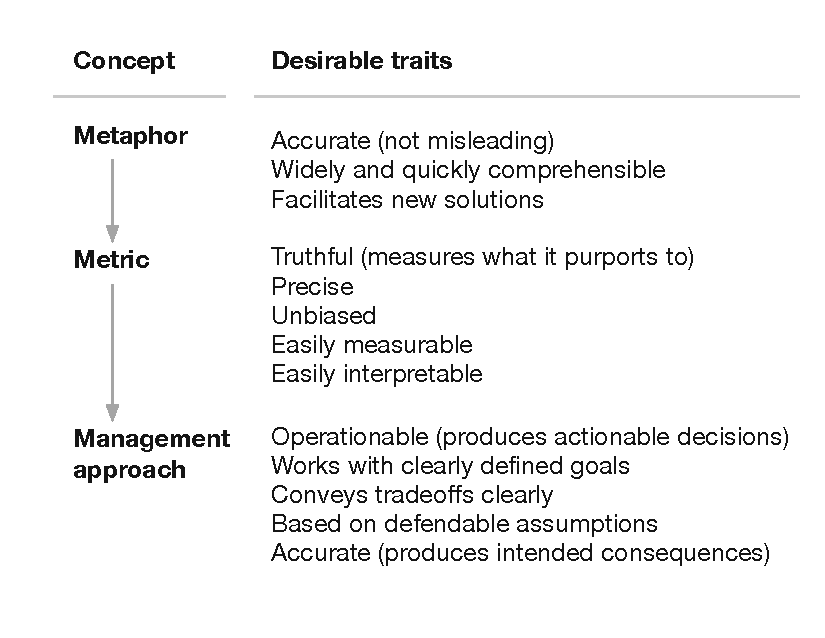
\includegraphics[width=4in]{mmm-traits.pdf}
\caption{Desirable traits of ecological metaphors, metrics, and management approaches
(decision-making tools).}
\label{fig:traits}
\end{figure}

But in applying financial theory to conservation biology, where does the portfolio metaphor break down? What exactly are the assets, portfolios, and investors in the financial metaphor? Furthermore, how might one invest in different kinds of ecological portfolios? And how might the differences between financial and ecological data affect our ability to apply financial portfolio theory to conservation biology? Are ecological portfolios just another name for existing ecological theory? Or, can ecological portfolios bring together and provide new insights into a wide variety of ecological theory?

TODO EDIT THIS!!! Here, we address these questions by reviewing the emerging literature on ecological portfolios. The purpose of our review is fourfold: review the three recent contrasting applications of ecological portfolios as metaphors, metrics, and management tools; illustrate how ecological portfolios can bring together a wide variety of modern ecological theory; highlight some challenges of applying financial theory to ecological portfolios; and emphasize the utility of portfolio optimization and risk metrics for conservation prioritization.

\section{Ecological portfolios as a metaphor}\label{ecological-portfolios-as-a-metaphor}

Metaphors are powerful tools for communicating and shaping scientific ideas \citep{brown2003} and are particularly useful in developing and communicating the field of conservation biology \citep{larson2011}. In conservation biology, the portfolio concept has long been used as a metaphor to emphasize the need to not put all your eggs in one basket. This metaphor has come into particular prominence in the last decade. For example, the IUCN Criterion B2a recognizes the risks associated with a species existing in few locations \citep{iucn2001}. As another example, ecologists have suggested the need to bet hedge by developping a portfolio of approaches when tackling conservation issues \citep[e.g.][]{ehrlich2008}. Ecologists have also used the metaphor to refer to diverse ecosystems and communities as portfolios of species \citep{figge2004}. These applications are an appealing way to convey concepts of diversification, uncertainty, and risk using familiar terminology.

\section{The portfolio-effect metric}\label{the-portfolio-effect-metric}

Beyond the metaphor, the portfolio-effect metric asks what the precise benefit is of a unit increase in diversity. The portfolio effect is derived from the economic question: How much better off are you by investing your money in a diversified portfolio instead of investing all your money in a single asset \citep{markowitz1952}? In conservation biology, we can consider the current ecological system the diversified portfolio and a theoretical homogeneous (or monoculture) system the single asset \citep{anderson2013}. For example, we could ask how much more stable is a metapopulation of salmon from different streams, rivers, or watersheds (the portfolio) compared to a theoretical homogeneous stream population (the single asset) \citep{schindler2010, carlson2011}. Hence, to accurately measure a portfolio effect we need to predict the variability of a theoretical homogeneous system---a system that lacks the element of biodiversity we are interested in. Unfortunately, although the portfolio metaphor provides a new way of looking at the decades-old diversity-stability debate, on its own it remains unclear whether it provides new insights about the nature of the relationship itself.

Nonetheless, by providing a new lens, the portfolio effect as a metric has created an impetus for new theoretical and empirical insights into stability-diversity relationships. Early work focused on theoretical aspects of the portfolio effect for greatly simplified systems---identifying when we would expect a stabilizing portfolio effect and what factors would enhance it \citep{doak1998, tilman1998, lehman2000}. Over time, theoretical studies developed indices that relaxed assumptions about the systems they describe \citep[e.g.][]{loreau2010a, thibaut2013, gross2013}. A recent trend has been to apply these indices to empirical data, albeit primarily to salmon \citep{greene2010, schindler2010, carlson2011, anderson2013, mellin2014}. However, empirical work has concentrated on applying relatively simple portfolio-effect metrics that make strong assumptions that are rarely met in empirical systems \citep{thibaut2013, anderson2013}. Violation of these assumptions, for example, the assumption that the temporal standard deviation scales directly with the mean, or that populations are approximately equal in size, can distort our perception of the portfolio effect and hence the perceived benefit of diversity to ecological stability \citep{anderson2013}.

\section{Ecological portfolio management}\label{ecological-portfolio-management}

In addition to measuring the portfolio-effect metric, we can use financial portfolio theory to inform decisions about conservation management. Markowitz's seminal contribution to financial portfolio theory was a focus on portfolio selection---the idea that out of all possible portfolios there exists a subset that maximize returns for a level of risk (or minimize risk for a level of return) \citep{markowitz1952} (Fig.~\ref{fig:mpt}). In conservation biology, the goals of conservation practitioners often parallel those of financial managers, even though they are rarely expressed as such \citep{figge2004}. We see ecological portfolio management happening in one of three ways: choosing existing management structures that promote diversified portfolios, using Modern Portfolio Theory (MPT) to optimize ecological resource extraction, or using MPT to optimize an ecological system itself.

\begin{figure}[htbp]
\centering
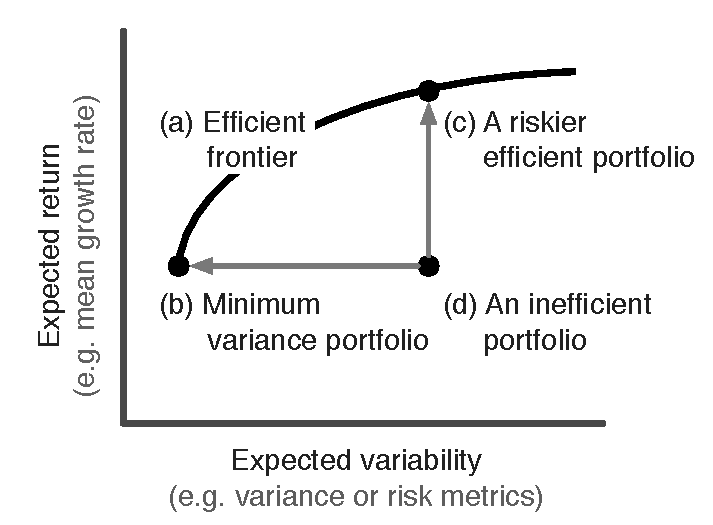
\includegraphics[width=3in]{efficient-frontier-fig.pdf}
\caption[An introduction to Modern Portfolio Theory mean-variance optimization.]{
An introduction to Modern Portfolio Theory mean-variance optimization. In
finance, portfolios are formed by choosing how much to invest in various
assets. Modern Portfolio Theory focuses on identifying the set of portfolios
that optimizes the trade-off between expected return (mean) and expected
variance or risk. (a) This set of portfolios is referred to as the efficient
frontier. (b) The minimum variance portfolio achieves the lowest expected
risk; the remaining risk is said to be undiversifiable. (c) A risker, but
still efficient portfolio. (d) An example inefficient portfolio, which has a
lower expected return than (c) and greater expected risk than (b). Adapted
from \citeauthor{hoekstra2012} (\citeyear{hoekstra2012}).
}
\label{fig:mpt}
\end{figure}

First, we can consider existing management structures that create systems analogous to diversified portfolios. For example, fishers can engage in catch-pooling cooperatives where fishers share the profits from their catches according to predefined rules. \citet{sethi2012} showed that this portfolio-like scheme reduces risk for red king crab fishers in the Bering Sea by up to 40\%. Other fisheries management tools, such as community-based management, individual transferable quotas (ITQs), and licensing systems that allow for fishing a diversity of species, can create diversified catch portfolios for fishers and buffer fishers against the risk of poor profits \citep{hilborn2001, kasperski2013}. Alternatively, we can consider the properties of a diversified portfolio, such as representation, resilience, and redundancy, and look for management strategies that promote these properties in ecological systems \citep{haak2012}

We can also use MPT directly to optimally allocate harvesting efforts. This suggestion is not new---some of the earliest references to ecological portfolios suggest portfolio theory as a management tool \citep{baldursson1997, costanza2000} but few studies have explored the idea to its full extent and interest in the topic has expanded strongly in recent years \citep[e.g.][]{edwards2004, sanchirico2008, halpern2011, moloney2011}. In conservation biology, portfolio optimization can be applied spatially. For example, \citet{halpern2011} used MPT to illustrate the tradeoff between fishing profits and spatial unevenness of marine resource value. MPT has also been used to optimize decisions about whether to clearcut or retain standing trees \citep{hyytiainen2008, hildebrandt2011}. As a third example, \citet{moloney2011} used MPT to optimize the choice of grazing animals on Australia's rangelands. With few exceptions, however, the application of MPT for harvesting decisions has been limited to fishery and forestry examples.

Finally, we can use ecological portfolio management to choose how we allocate conservation efforts to manage risk for an ecological system as a whole. For example, portfolio optimization can be used to spatially allocate conservation activity for wetlands to maximize ecosystem services at a given level of risk under the uncertainty of climate change \citep{ando2011, ando2012}. In forestry, MPT has been used to select the optimal weighting of seed sources for regenerating forests under a variety of climate change scenarios \citep{crowe2008}. In fisheries, MPT has been used to assess the risk-return trade-off for salmon metapopulation productivity given choices about what habitat to conserve under climate change and stream-flow reduction scenarios \citep{anderson2014}. We see this as a promising but largely unexplored use of ecological portfolio theory.

\section{Ecological theory to draw from}\label{ecological-theory-to-draw-from}

Portfolio theory can unite many existing ecological theories (Table~\ref{tab:theory}). For example, community ecology, the theory of island biogeography, metapopulation dynamics, and functional-group ecology can all generate portfolio-like ecological structure. Importantly, the portfolios produced by these scenarios have specific features that affect portfolio dynamics. For example, in community portfolios, predator assets can eat portions of prey assets, which has no direct equivalent in financial portfolios. In metapopulation portfolios, subpopulation assets can exchange individuals between each other and rescue subpopulation assets at low abundance or value.

Other ecological theories can inform expected patterns of diversification and portfolio dynamics (Table~\ref{tab:theory}). For instance, the Moran effect suggests that ecological assets that are further apart from each other are more likely to experience diverse environments and therefore provide greater portfolio diversification. The unified neutral theory of biodiversity and biogeography asks what we would observe if species were functionally equivalent. We can think of this neutral community as an undiversified portfolio and compare it to observed communities to examine the benefit of functional diversity. This comparison is analogous to the ecological portfolio-effect metric \citep[e.g.][]{doak1998, schindler2010, anderson2015}.

Finally, a variety of mechanisms can generate ecological portfolio diversification (Table~\ref{tab:theory}). For instance, intraspecific trait variation, response diversity, and even personality variation can be thought of as sources of portfolio diversification. Ecological portfolios therefore can have multiple levels of diversification, just as financial portfolios can be diversified across multiple levels such as investment types, geography, business sectors, and individual stocks. Whereas research on many of these ecological sources of diversification exists in its own niche, ecological portfolio theory encourages us to consider many elements in conjunction.

\LTcapwidth=\textwidth
\bibpunct{}{}{;}{a}{}{;}
%\singlespacing
\begin{small}
\begin{longtable}{>{\RaggedRight}p{3.6cm}>{\RaggedRight}p{7.3cm}>{\RaggedRight}p{3.6cm}}

\caption{Selected ecological theory relevant to ecological portfolios.}\\

\toprule

\textbf{Ecological theory} &
\textbf{Relevance to ecological portfolios} &
\textbf{Selected references} \\

\midrule
\multicolumn{2}{l}{\textbf{Sources of portfolio structure}} \\
\midrule

Community ecology &
We can represent species as assets and a community as a portfolio. Species interactions such as predation and competition may complicate the analogy. &
\citep{figge2004, morin2011}\\

Theory of island biogeography &
Explains a source of diversification for ``islands'', which have a portfolio-like structure. Larger islands may have higher levels of portfolio diversification. &
\citep{macarthur1967}\\

Metapopulations &
Subpopulations can act as diverse ecological assets as part of a metapopulation portfolio. Metapopulations usually have exchange between subpopulations (ecological assets), which may not have an analogy in financial portfolios. &
\citep{levins1969}\\

Functional groups &
Species that perform separate ecological functions can form ecological assets as part of an ecological portfolio. &
\citep{walker1992, thibaut2012}\\

\midrule
\multicolumn{2}{l}{\textbf{Causes of diversification and portfolio dynamics}}\\
\midrule

Moran effect &
Identifies that similar environments will induce similar population responses decreasing the diversity of a portfolio. Ecological assets that are further apart are expected to provide greater diversification. &
\citep{moran1949, ranta1998}\\

\bibpunct{(}{)}{;}{a}{}{} % add back brackets for in-text citation
Synchrony &
Often loosely used to referred to as correlation between ecological assets. Defined quantitatively by \citet{loreau2008} as a diversity-independent metric of correlation. The benefit of diversification is greater when synchrony of ecological assets is low. &%
\bibpunct{}{}{;}{a}{}{}%
\citep{ranta1998,moore2010,yeakel2014}\\

Unified neutral theory of biodiversity and biogeography &
Asks what community dynamics we would observe if species were functionally equivalent. We can think of a neutral community with ecological equivalence as an un-diversified portfolio compared to a diversified portfolio in which species show functional diversity. &
\citep{hubbell2001}\\

Biocomplexity &
Identifies that subpopulations can display a range of biological traits and behaviours and that these ranges can form portfolio diversification &
\citep{hilborn2003, hutchinson2008}\\

Response diversity &
Identifies elements of ecological systems that cause them to respond differently to perturbation. Potentially important aspect of ensuring stable portfolios as the magnitude and frequency of environmental stressors increase (e.g.\ climate change). &
\citep{elmqvist2003, loreau2008, loreau2013}\\

Intraspecific trait variation &
Identifies that variation among individuals in a population can form an important component of diversity and affect population dynamics. Individuals could be thought of as ecological assets. &
\citep{bolnick2011}\\

Spatial heterogeneity &
Heterogeneity in habitat may create pockets of diverse ecological assets. &
\citep{oliver2010,parn2012,mccluney2014}\\

%Compensatory dynamics and complementarity & … & [65]\\

%Competitive interactions & … & [37]\\

\midrule
\multicolumn{2}{l}{\textbf{Risk-reduction consequences of diversity}}\\
\midrule

Diversity-stability hypothesis &
Identifies when and why certain types of diversity correspond with certain types of stability. Another name for many of the same concepts that ecological portfolio theory addresses.  &
\citep{ives2007, loreau2013}\\

Statistical averaging &
Some level of reduction in variability in a portfolio is inevitable due to averaging of asset time series. &
\citep{doak1998}\\

Portfolio effect &
A term to represent the benefit of a system existing as a portfolio of ecological assets instead of a single homogeneous asset. &
\citep{tilman1998, schindler2010, thibaut2013, anderson2013}\\

Insurance hypothesis &
Similar to the portfolio effect, but emphasizes that negative covariance reduces the likelihood that all assets will decline at the same time. &
\citep{yachi1999,valone2008}\\

\bottomrule
\label{tab:theory}
\end{longtable}
\end{small}


TODO introduce the data chapters here

\bibliographystyle{apalike}\bibliography{/Users/seananderson/Dropbox/tex/jshort,/Users/seananderson/Dropbox/tex/ref3}
